
\usepackage{fancyhdr}
\usepackage{lastpage}
\usepackage[utf8]{inputenc}

% Minted for syntax highliting
\usepackage{minted}
\usemintedstyle{tango}

% 
\usepackage[T1]{fontenc}
\usepackage{lmodern}

\usepackage{calc}
\usepackage{bytefield}

\usepackage{listings}
\usepackage{amsmath}

\usepackage{tikz}
\usetikzlibrary{automata,arrows,topaths,calc,positioning}
 
\usepackage{syntax}
\grammarindent=2cm


% Headers/footers styling
\pagestyle{fancy}
\fancyhf{}
\renewcommand{\headrulewidth}{0pt}

% Footer
\lfoot{ID1019}
\cfoot{KTH}
\rfoot{\thepage \hspace{1pt} / \pageref{LastPage}}

%\newcommand{\defaultpagestyle}{\thispagestyle{plain}}
\newcommand{\defaultpagestyle}{\thispagestyle{fancy}}



\usepackage{pgf-umlsd}
\usepgflibrary{arrows} % for pgf-umlsd

\title[ID1019 A transport layer]{A game of Pong}


\author{Johan Montelius}
\institute{KTH}
\date{\semester}

\begin{document}

\begin{frame}
\titlepage
\end{frame}

\begin{frame}{the classical game of Pong}

  \begin{figure}
    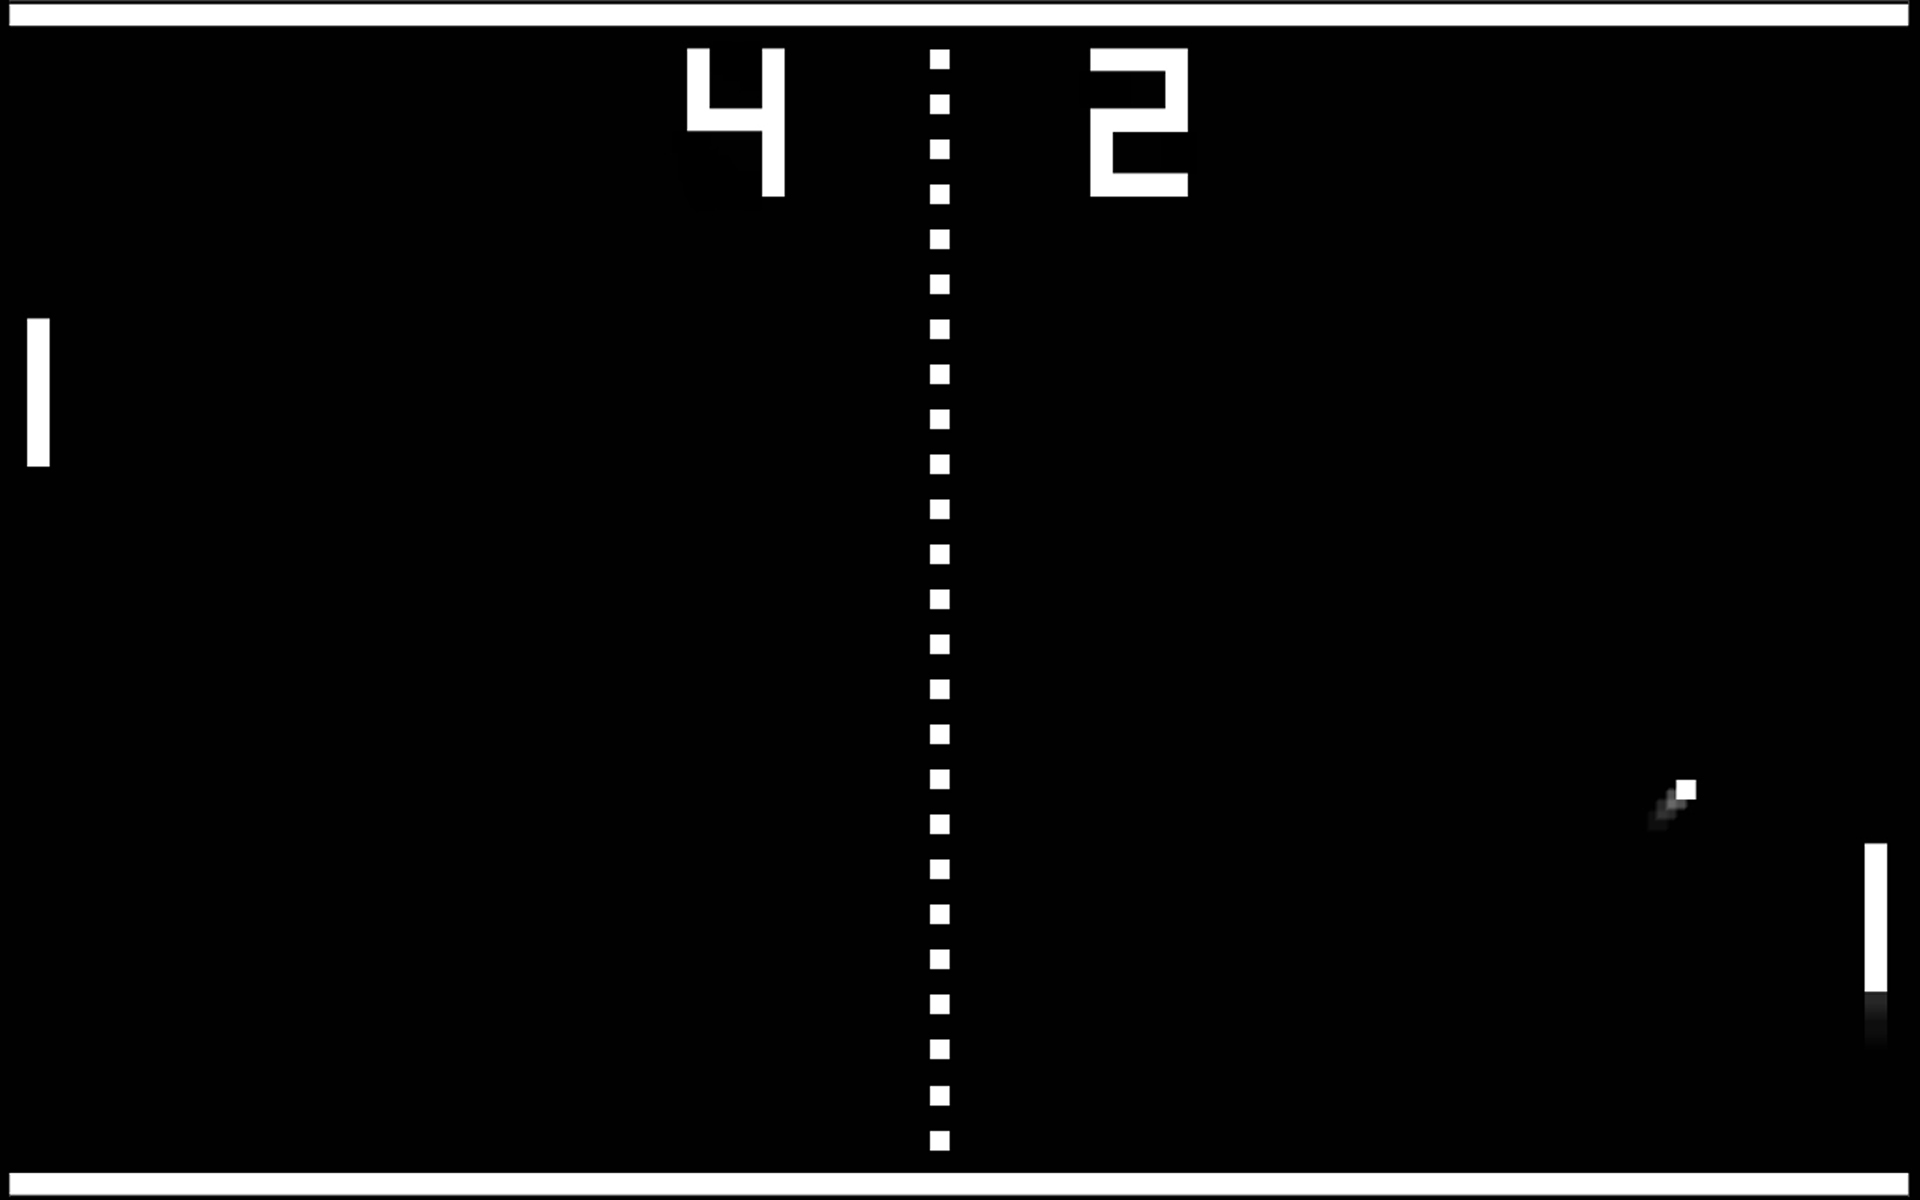
\includegraphics[scale=0.4]{pong.png}
  \end{figure}
  
\end{frame}

\begin{frame}{architecture overview}


\begin{figure}
\begin{tikzpicture}

  \coordinate (n0) at (0,6);
  \coordinate (nn) at (0,-0.5);

  \coordinate (a0) at (3, 3);
  \coordinate (an) at (3,-0.5);

  \coordinate (b0) at (5,4);
  \coordinate (bn) at (5,-0.5);

  \coordinate (c0) at (7,5);
  \coordinate (cn) at (7,-0.5);

  \coordinate (s0) at (12,6);
  \coordinate (sn) at (12,-0.5);


  \draw[->] (n0) to []  (nn);
  \draw[->] (s0) to []  (sn);

  \node[anchor=south] at (n0) {browser};
  \node[anchor=south] at (s0) {pong server};

  \pause

  \pause
  \coordinate (s2) at ($(s0)+(0,-1)$);
  \draw[dashed] (s2) -- node[near start, above]{start(name, me)\ \ } (c0);
  \node[anchor=south] at (c0) {ses1/2};  
  \draw[->] (c0) to []  (cn);

  \pause
  
  \coordinate (s3) at ($(s2)+(0,-1)$);
  \draw[dashed] (s3) -- node[near start, above]{start(8080,[ses1, ses2])\ \ } (b0);
  \node[anchor=south] at (b0) {srv};  
  \draw[] (b0) to []  ($(b0)+(0,-2)$);

  \pause

  \coordinate (b1) at ($(b0)+(0,-1)$);
  \draw[dashed] (b1) -- (a0);        
  \node[anchor=south] at (a0) {hdlr1/2};  
  \draw[->] (a0) to []  (an);  

  \pause

  \coordinate (n4) at ($(n0)+(0,-4)$);
  \coordinate (a1) at ($(a0)+(0,-1)$);
  \draw[dashed, <->, shorten <=0.2cm, shorten >=0.2cm] (n4) -- node[midway, above] {websocket} (a1);

  \pause
  \coordinate (a2) at ($(a1)+(0,-1)$);
  \coordinate (c2) at ($(c0)+(0,-4)$);
  \draw[->, shorten <=0.2cm, shorten >=0.2cm] (a2) -- node[midway, above] {\{:ws, pid, :open\}} (c2);

  \pause
  \coordinate (c3) at ($(c2)+(0,-1)$);
  \coordinate (s4) at ($(s3)+(0,-4)$);
  \draw[->, shorten <=0.2cm, shorten >=0.2cm] (c3) -- node[midway, above] {\{:ready, name\}} (s4);  


\end{tikzpicture}

\end{figure}
\end{frame}


\begin{frame}{WebSocket interface}

  The Javascript client communicte using a websocket interface. After
  the initial HTTP handshake, a birectional message channel is
  created. Each message consist of sequence of bytes.

  \pause\vspace{10pt}
  
  
  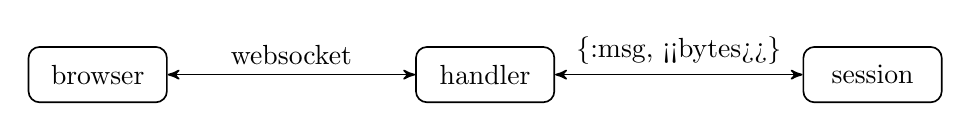
\begin{tikzpicture}[>=stealth', node distance=140pt, semithick, auto]

        \tikzstyle{fbp} = [rectangle, rounded corners, minimum width=50pt, minimum height=20pt,text centered, draw=black]        

        \node (brw1) [fbp] {browser};
        \node (hdlr1) [fbp, right of=brw1] {handler};

        \path[<->]  (brw1) edge   node      {websocket}       (hdlr1);
        \pause
        \node (ses1) [fbp, right of=hdlr1] {session};
        \path[<->]  (hdlr1) edge   node      {\{:msg, <<bytes>>\}}       (ses1);

\end{tikzpicture}

  \pause\vspace{10pt}
  
  The websocket handler process will take care of the wesocket
  internals and deliver a stream of messages to the session process.

  \pause

  Each client is connected through a unique handler process that is
  communicating with a single session process.

\end{frame}

\begin{frame}{Session handler lower interface}

Messages from the websocket handler process:

\vspace{10pt}  \pause

\begin{itemize}
\item {\tt \{:ws, pid, :open\}}  : a connection was establishes
\item {\tt \{:ws, pid, :close\}}  : the connection was closed by the client
\item {\tt \{:ws, pid, \{:msg,  <<byte encoded message>>\}\}} : message from the client
\end{itemize}

\vspace{10pt}  \pause

Messages to the websocket handler process:

\begin{itemize}
\item {\tt \{:frw, <<byte encoded message>>\}}  : encode and send message to client
\item {\tt :stop} : time to close the connection
\end{itemize}

\end{frame}

\begin{frame}{The session handler}

  Works as a deocer/encoder of byte-encoded  messages and Elixir messages.

  \vspace{20pt}  \pause

  Messages from the client forwarded to the pong game server:

  \vspace{20pt}

  \begin{itemize}
  \item {\tt <<?U>>}  : player pressed up -  {\tt \{name, :up\}}
  \item {\tt <<?D>>}  : player pressed down -  {\tt \{name, :down\}}        
  \end{itemize}


\end{frame}

\begin{frame}{session handler}

  Messages from pong server fowarded to the websocket handler:

  \vspace{20pt}
      
  \begin{itemize}
  \item {\tt \{:player1, :up\}}  : player moved up -  {\tt <<?P,?U>>}
  \item {\tt \{:player1, :down\}}  : player moved down - {\tt <<?P,?D>>}
  \item {\tt \{:player1, :score, score\}}  : player moved up - {\tt <<?P,?S, score>>}
  \item {\tt \{:player2, ... \}} : same messages for opponent -  {\tt <<?O, ... >>}        
  \item {\tt \{:ball, x, y \}} : ball moved to new position - {\tt <<?B, x::16, y::16 >>}        
  \item {\tt \{:frw, msg\}}  : raw message to client - {\tt msg}
  \end{itemize}
\end{frame}

\begin{frame}{the game engine}

  The game server:
  \vspace{10pt} \pause
  \begin{itemize}
  \item create two session handlers with unique names \pause
  \item create a WebSocket process, give session handlers as arguments \pause
  \item wait for session handlers to report \pause
  \item sart the game \pause
  \end{itemize}
  
\end{frame}


\begin{frame}{the game engine}

  The pong engine keeps a state consisting of:

  \vspace{10pt} \pause
  
  \begin{itemize}
  \item Two players ({\tt player1} and {\tt player2}) that have a {\em y-position} and a {\em score}. \pause
  \item A ball that is defined by {\em x-} and {\em y-position}, and {\em x-} and {\em y-speed}.\pause
  \item Two {\em session pids} to send messages to the players. 
  \end{itemize}

  \vspace{10pt} \pause

  The pong engine is defined by two modules: 
  
  \vspace{10pt} \pause
  \begin{itemize}
  \item The Pong module that describes the server as a communicatng process. 
  \item The Game module that describe the rules as functions. 
  \end{itemize}
  

\end{frame}
  
  


\end{document}



